\section{Размерное квантование}
Квантоворазмерный эффект (квантовый размерный эффект) — изменение термодинамических и кинетических свойств кристалла, когда хотя бы один из его геометрических размеров становится соизмеримым с длиной волны де Бройля электронов. Этот эффект связан с квантованием энергии носителей заряда, движение которых ограничено в одном, двух или трёх направлениях.\\

Волны де Бройля — волны вероятности, определяющие плотность вероятности обнаружения объекта в заданной точке конфигурационного пространства. В соответствии с принятой терминологией говорят, что волны де Бройля связаны с любыми частицами и отражают их волновую природу.

\begin{gather} 
	\lambda = \frac{h}{p} = \frac{h}{\hbar k} = \frac{h}{mv};\\
	\psi(x, t) = A*e^{\frac{i}{\hbar}(px-Et)} = A*e^{i(kx-\omega t)}.
\end{gather}

В зависимости от размерности пространства электронный газ имеет различный закон дисперсии, плотность состояний и эффективную плотность состояний, см табл.~\ref{tab:gE} \cite{Harrison}.

\begin{center}
    \begin{longtable}{| c | c | c | c |}
	    \caption{Плотность состояний и эффективная плотность состояний для низкоразмерных систем}
	    \label{tab:gE}
	    \\ \hline
	    Размерность & Закон дисперсии & $g(E)$ & $G(E)$ \\
	    \hline \endfirsthead
	    \subcaption{Продолжение таблицы~\ref{tab:gE}}
	    \\ \hline \endhead
	    \hline \subcaption{Продолжение на след. стр.}
	    \endfoot
	    \hline \endlastfoot
	    3D, bulk & $\frac{\hbar^{2}}{2m}(k_{x}^{2}+k_{y}^{2}+k_{z}^{2})$ & $ \frac{2^{\frac{1}{2}}m^{\frac{3}{2}}}{\pi^{2}\hbar^{3}}E^{\frac{1}{2}} $ & $\frac{(2m)^{\frac{3}{2}}}{3\pi^{2}\hbar^{3}}E^{\frac{3}{2}}$\\
	    \hline
	    2D, well & $\frac{\hbar^{2}}{2m}(k_{x}^{2}+k_{y}^{2})+\frac{\pi^{2}\hbar^{2}n^{2}}{2mL^{2}}$ & $\frac{m}{\pi\hbar^{2}}$ & $\frac{m}{\pi\hbar^{2}}E$\\
	    \hline
	    1D, wire & $\frac{\hbar^{2}}{2m}(k_{x}^{2}) + \frac{\pi^{2}\hbar^{2}}{2m}\Big( \frac{n_{1}^{2}}{L_{1}^{2}} + \frac{n_{2}^{2}}{L_{2}^{2}} \Big)$ & $\frac{\sqrt{m}}{\sqrt{2}\pi\hbar}E^{-\frac{1}{2}}$ & $\frac{\sqrt{2m}}{\pi\hbar}E^{\frac{1}{2}}$\\
	    \hline
	    0D, dot & $\frac{\pi^{2}\hbar^{2}}{2m}\Big( \frac{n_{1}^{2}}{L_{1}^{2}} + \frac{n_{2}^{2}}{L_{2}^{2}} + \frac{n_{3}^{2}}{L_{3}^{2}} \Big)$ & $2\delta E$ & $2$
    \end{longtable}
\end{center}

\begin{figure}[h]
	\centering
	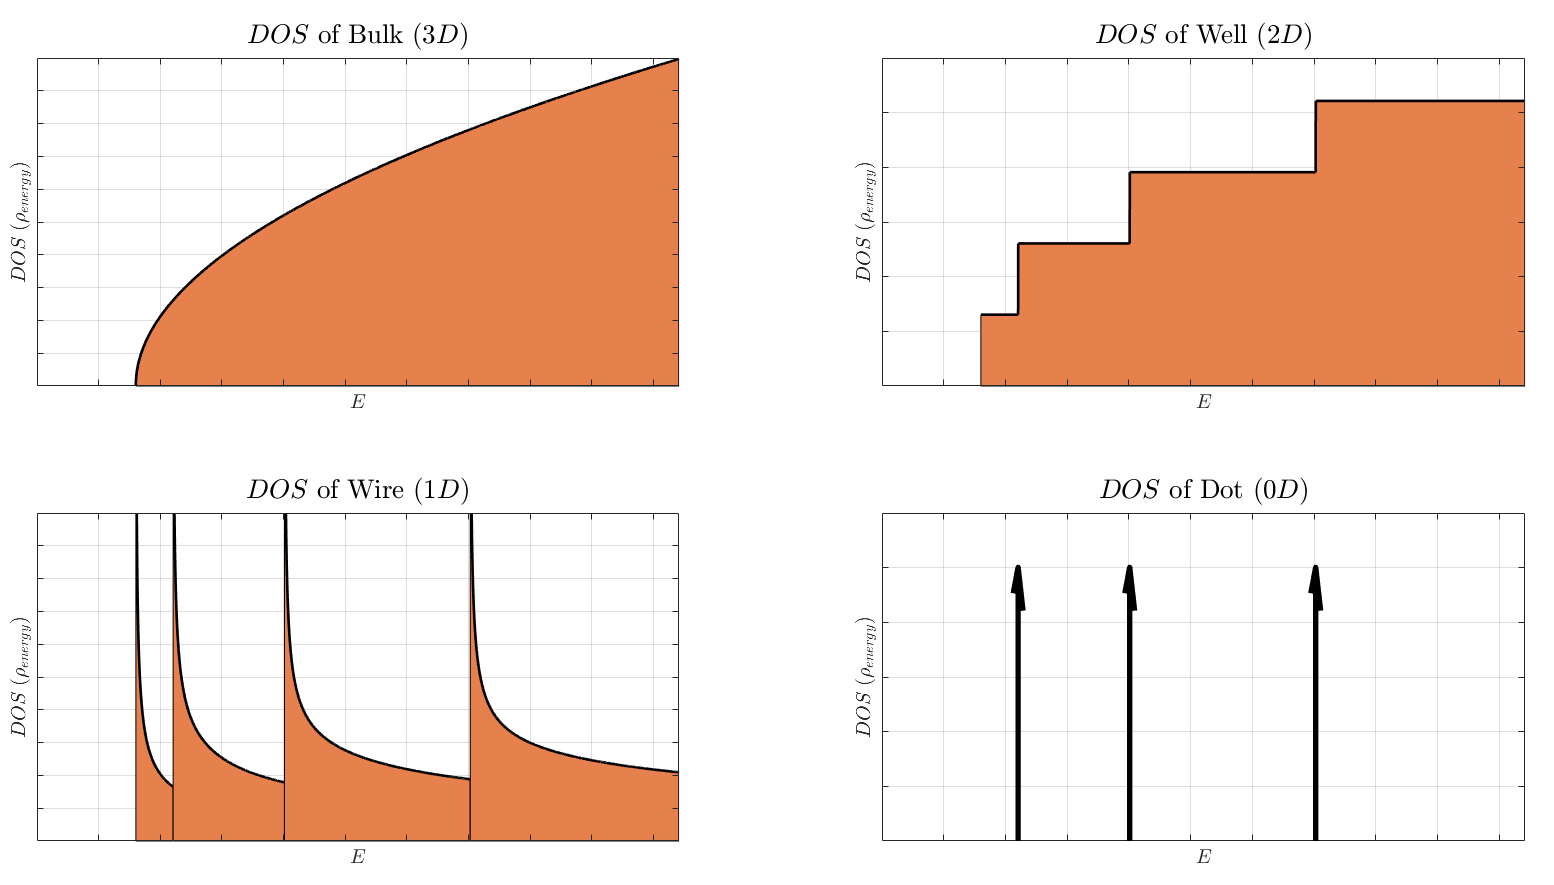
\includegraphics[width=\textwidth]{gE.png}
	\caption{Плотность состояний в 3D, 2D, 1D, 0D, где $g(E) = \rho_{energy}$}
	\label{DOS}
\end{figure}

\subsection{Трехмерное тело}
Рассмотрим 3D кристалл (bulk) на рис.~\ref{fig:3DBulk}:
\begin{figure}[h]
	\centering
	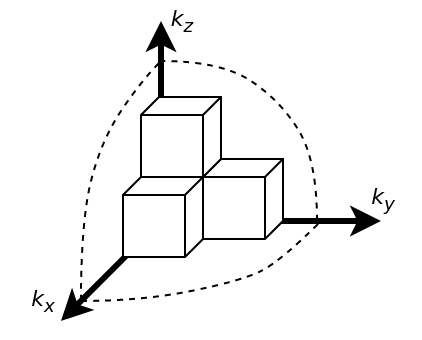
\includegraphics[scale=0.5]{3DBulk.png}
	\caption{k-пространство (шар)}
	\label{fig:3DBulk}
\end{figure}

Число состояний частицы $G(E)$ и плотность состояний $g(E)$, энергия которых не превышает некоторого фиксированного значения $E$, находятся из формул:
\begin{gather*} 
	G(E) = \frac{V_{sphere}}{V_{single-state}} = J_{z}\frac{\frac{1}{8}\frac{4}{3}\pi k^{3}}{\frac{\pi^3}{V}} = \frac{k^{3}V}{3\pi^{2}} = \frac{(2m)^{\frac{3}{2}}V}{3\pi^{2}\hbar^{3}}E^{\frac{3}{2}};\\
	k = \frac{\sqrt{2mE}}{\hbar};\\
	g(E) = \frac{dG(E)}{dE} = \frac{(2E)^{\frac{1}{2}}m^{\frac{3}{2}}}{\pi^{2}\hbar^{3}}V.
\end{gather*}

\subsection{Двухмерное тело}
Рассмотрим 2D кристалл (well) на рис.~\ref{fig:2DWire}:
\begin{figure}[h]
	\centering
	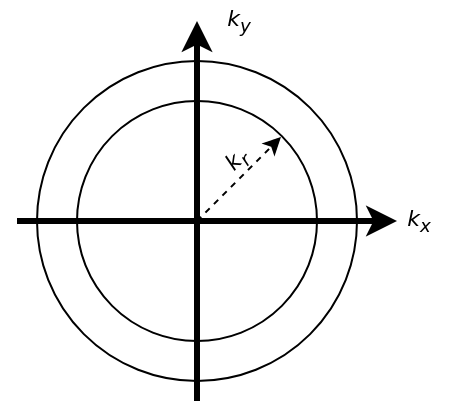
\includegraphics[scale=0.5]{2DWire.png}
	\caption{k-пространство (круг)}
	\label{fig:2DWire}
\end{figure}

\begin{gather*} 
	G(E) = \frac{V_{circul}}{V_{single-state}} = J_{z}\frac{\frac{1}{4}\pi k^{2}}{\frac{\pi^2}{S}} = \frac{k^{2}}{2\pi} = \frac{mS}{\pi\hbar^{2}}E;\\
	g(E) = \frac{dG(E)}{dE} = \frac{m}{\pi\hbar^{2}}S.
\end{gather*}

\subsection{Одномерное тело}
Рассмотрим 1D кристалл (wire)  на рис.~\ref{fig:1Ddot}:
\begin{figure}[h]
	\centering
	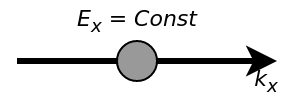
\includegraphics[scale=0.5]{1Ddot.png}
	\caption{k-пространство (линия)}
	\label{fig:1Ddot}
\end{figure}
\begin{gather*} 
	G(E) = \frac{V_{line}}{V_{single-state}} = J_{z}\frac{k}{\frac{\pi}{L}} = \frac{kL}{pi} = \frac{\sqrt{2m}L}{\pi\hbar}E^{\frac{1}{2}};\\
	g(E) = \frac{dG(E)}{dE} = \frac{\sqrt{m}L}{\sqrt{2}\pi\hbar}E^{-\frac{1}{2}}.
\end{gather*}

$J_{z}$ -- определяет число состояний не связанных с перемещением частицы в пространстве (например, число возможных проекций спина). В нашем случае, для электрона $J_{z}=2$.